\documentclass{report}
\usepackage[margin=1.25in]{geometry}
\usepackage[sc]{mathpazo}
\linespread{1.05}
\usepackage[T1]{fontenc}

\usepackage{nicefrac}
\usepackage{amsmath}
\usepackage{amssymb}
\usepackage{url}
\usepackage{natbib}
\usepackage{graphicx}
\usepackage{caption}

\begin{document}
\title{Computing a Feasible Trajectory Through an Obstacle Field Using Nonlinear Constrained Optimization}
\author{
    Simon Broadhead\\
    Jeremy Ciesinski\\
    J.D. Cumpson\\
    Craig Skelsey\\
    Peter Smyth\\
    Junaid Syed\\
    Subramanian Venkatesan
}
\maketitle

\tableofcontents

%%%%%
\chapter{Problem Overview}
\section{A Pathfinding Problem}
Pathfinding is a very important topic in the field of Computer Science.
Generally, when we talk about pathfinding algorithms, we talk about
algorithms to find the optimal path (for some objective function) through
a graph from a source vertex to a destination vertex. Even in
non-graph contexts---for example in video games---the more general problem
of finding a path through Euclidian space is often restricted to a graph
for simplicity.

But what if the problem is not able to be solved in this way? What if
we want to find a path between two points through a series of obstacles,
but without foreknowledge of the layout? That is, the only information
that we have is the information that we can currently see. Furthermore,
what if we cannot control our position directly, but can only control
some other parameters? Then the problem becomes much trickier.
\vspace{0.5em}

Consider the following problem:
\vspace{0.5em}

You have a circular spaceship with radius $r$ and mass $m$
in two dimensions located at some point $\mathbf{p}$ equipped with thrusters
on a pair of antipodal points. There
is a known point $\mathbf{q}$ somewhere on the plane, and you want to
get the spaceship there in a reasonable amount of time. Also present
in the space are large polygonal obstacles (e.g., asteroids) 
that must be avoided en route
to $\mathbf{q}$. Although you know where $\mathbf{q}$ is in relation to
$\mathbf{p}$, you don't know where the obstacles are, aside from the
points that you can actually see.

The only way to move the ship is to turn the thrusters up or down. 
For the purposes of this problem, the thrusters are infinitely small
and lie extactly on the circumference of the ship, with thrust being
applied tangentially.
To
move forward, set them to an equal positive force. To move backward,
set them to an equal negative force. To spin around,
the sum should be zero. There is no
way to directly control where in space the ship is at any given time,
or even how fast it is moving; only the acceleration can be controlled
directly, by the thrusters. The thrusters must also be gradually changed
over time; they cannot jump instantly from 10 Newtons to $-10$ Newtons,
for example.
\vspace{0.5em}

In this report, we will attempt to describe a method of solving this
problem using nonlinear optimization methods.

\section{A Piecewise Approach}
Taken as a whole, this problem does not lend itself well to numerical
optimization. The problem itself is inherently non-convex due to the
feasible space having holes in it where the obstacles are, so it is likely
that a solution could not even be found using the usual constrained
optimization methods.

There is, however, a simpler problem that we \emph{can} solve with
constrained optimization, and it happens to be a natural subproblem of
the problem we are really trying to solve. Consider the original
problem, except without any obstacles; we want to compute a trajectory
between two points \emph{within a convex region}. If we can do that,
then we can break the original feasible problem space into convex
regions and solve the subproblem within each region. We can then focus
on solving two separate problems: determining the convex subregions, and 
finding a feasible trajectory within each.

We want to guarantee that the ship doesn't crash, but since we can't see
into the future (at least not beyond the end of the current subproblem),
we need to impose a constraint on the subproblems that
may at first seem drastic:
within each convex subregion, the trajectory from $\mathbf{p}$ to
$\mathbf{q}$ must come to a stop at the end. That doesn't mean, however, that the
ship will be frequently stopping and starting during its journey;
computing such a trajectory only proves that it \emph{can} stop. If we
follow our computed trajectory for only a short amount of time before
throwing it out and solving a new subproblem---hopefully with some new
information each time---we can keep moving closer and closer to the
destination, all the while knowing that we can stop if we must.


%%%%%

\chapter{Finding a Trajectory in a Convex Region}
The majority of the work we did focused on the subproblem of finding feasible
trajectories within a convex region. This is the aspect of the problem that utilizes
continuous nonlinear optimization methods and so this is where we devoted most
of our time.
\section{Modeling the Thrust Profile}
Since this is an optimization problem over time, we must decide how we will encode
the passage of time within the problem. In particular, we must decide how we will
determine the amount of thrust that should be applied by the left and right thrusters
at each point in the time interval.

We must define a pair of thrust profile functions
\[ f_L(t), f_R(t) : \mathbb{R} \to \mathbb{R}. \]
That is, for each time, we have two real numbers representing the force from the left and right
thrusters.
This function would ideally be simple and characterized by a relatively small number of variables (i.e.,
a low-degree polynomial).

We did not have time to explore the general case of this function. For example two functions of the form
\[ t \mapsto \alpha_0 + \alpha_1 t + \alpha_2 t^2 + \alpha_3 \sin(\alpha_4 t) \]
might be sufficient to model the type of simple motion we would like the solver to generate.

Generally the trajectory we are looking can be divided roughly into
two phases: correcting the existing momentum to accelerate towards the target point, and 
decelerating to come to a stop at the end of the interval. In this case, the trajectory
might be represented as a spline made up of one polynomial for each phase.

For simplicity, however, we chose to represent the thrust profile as a piecewise constant
function. In this model, there are two different ways we can discretise the time domain:
fixed time steps or variable time steps.

In the variable-time-step approach, the length of each time step is introduced as an additional
variable in the optimization problem. There are several benefits to this approach.
For one, it allows the solver to use the limited number of time steps more efficiently; in a
fixed-time-step approach, there may be a long stretch of time (say, half of the time steps)
during which the thrusters have very little variation from one step to the next followed by a
precise maneuver requiring rapid changes in the thrust levels. By using variable time steps,
the solver would be able to put the first part of the trajectory into one or two longer time steps
and use the remaining ones for more precise control over several small time steps.

Another benefit of the variable-time-step approach is that it allows direct measurement of the time
needed to complete the trajectory, which is simply the sum of each time step length.
With appropriate constraints on the trajectory (i.e., to prevent the ship from overshooting
or orbiting the target before reaching it) this could be used to have the solver minimize the 
length of the trajectory.

The obvious detriment to this approach is that for $N$ time steps, we are introducing $N$ new
variables to the problem. This makes the gradient of the objective function significantly
more expensive to calculate. Worse, this may introduce some severely non-convex behaviour
resulting the solver getting stuck in a local minimum. For a trivial example of non-convexity,
we can, given a trajectory that has
``left-over'' (i.e., zero-length) time steps at the end, construct an identical
trajectory by splitting one of the nonzero time steps into two identical time steps.

Ultimately, we decided on using the fixed-time-step approach. Not only did this simplify the
objective function considerably by converting many variables to constants, it also
gave better results in our experiments. We consider the constants $\Delta_t$ (the time step
length) and $N$ (the number of time steps) to be parameters of the optimization problem, to
be tuned for each instance of the problem.

Thus, we introduce the following parameters:

\begin{align*}
    \Delta_t \in \mathbb{R} &: \text{Length in seconds of one time step} \\
    N \in \mathbb{Z} &: \text{Total number of time steps}
\end{align*}

With that decision made, we can introduce the only independent variables in the problem:
\begin{alignat*}{3}
    & l_i \in \mathbb{R} &&: \text{Thrust in Newtons from the left thruster at time $i$} && \quad (1 \leq i \leq N) \\
    & r_i \in \mathbb{R} &&: \text{Thrust in Newtons from the right thruster at time $i$} && \quad (1 \leq i \leq N)
\end{alignat*}

\section{Modeling Motion} \label{sec:motion}
Having chosen a hopefully suitable thrust profile model, we must now figure out how to
convert that thrust into motion.

In our simplified physics model of the 2-d ship, we consider there to be no friction,
and that the mass does not change over time (i.e., from fuel loss).

First we will define a couple of parameters that characterize the physical properties of
the ship:
\begin{align*}
    M \in \mathbb{R} &: \text{Mass of the ship in kilograms} \\
    R \in \mathbb{R} &: \text{Radius if the ship in metres} \\
    \Delta_\text{thrust} \in \mathbb{R} &: \text{The maximum change in thrust per second}
\end{align*}

Since the only direct control we have over the ship's motion is by setting the force of the
left and right thrusters, we can represent the motion of the ship during time step $i$
as a system of differential
equations:
\begin{alignat*}{4}
    \omega'_i(t) &= \frac{2(l_i - r_i)}{MR} & \qquad \omega &: \text{angular velocity} \\
    \mathbf{d}'_i(t) &= \mathbf{d}_i^{\perp}(t) \omega(t) & \qquad \mathbf{d} &: \text{orientation unit vector} \\
    \mathbf{v}'_i(t) &= \frac{l_i + r_i}{M} \mathbf{d}_i(t) & \qquad \mathbf{v} &: \text{translational velocity} \\
    \mathbf{p}'_i(t) &= \mathbf{v}_i(t) & \qquad \mathbf{p} &: \text{position}
\end{alignat*}
In this system, $\mathbf{d}^{\perp}$ refers to the vector $(-d_y, d_x)$, a vector perpendicular to
the direction of the ship. 

There is no simple closed-form solution to this system, so we must approximate a solution
by discretising the system and solving it iteratively over much smaller time steps.

\subsection{Approximation by Finite Differences} \label{sec:linearapprox}
The most straightforward way to solve the system is by taking the variables to be piecewise constant.
By ignoring
variations within each time step,
we can approximate the solution over a time step by defining some step size $h \ll \Delta_t$
and iterating a finite difference approximation over the smaller steps.
If we choose a small enough step size that the behaviour of the
functions within each interval is nearly linear, we will achieve sufficient accuracy. We can approximate
the solution in time step $i$ with the following recurrence:
\begin{align*}
    \Delta\omega &= \frac{2(l_i - r_i)}{MR} \\
    \omega_k &= \omega_{k-1} + h \Delta\omega \\
    \theta &= \frac{h}{2} (\omega_{k-1} + \omega_k) \\
    \mathbf{d}_k &= \begin{bmatrix}\cos \theta & -\sin \theta \\ \sin \theta & \cos \theta\end{bmatrix} \mathbf{d}_{k-1} \\
    \mathbf{a}_k &= \frac{l_i + r_i}{M} \mathbf{d}_{k} \\
    \mathbf{v}_k &= \mathbf{v}_{k-1} + \mathbf{a}_{k-1} h \\
    \mathbf{p}_k &= \mathbf{p}_{k-1} + \mathbf{v}_{k-1} h + \frac{\mathbf{a}_{k-1}}{2} h^2
\end{align*}
Note that in this case $\omega_k$ is an exact solution, since $\omega' = \Delta\omega$ is a constant.

In practice, this gives good results for $h = \nicefrac{\Delta_t}{5}$, although we chose a
safer step size of $h = \nicefrac{\Delta_t}{10}$.


\subsection{Power Series Approximation of System} \label{sec:power}
Although the approximation model given in Section~\ref{sec:linearapprox}
achieves good results, we wanted to try to find a model that would not ignore higher-order
variation in the solution.

Expanding the $\mathbf{d}^{\perp}$ notation,
the direction component of the movement is given by a pair of
coupled differential equations
\begin{equation} \label{eq:orig}
    \begin{aligned}
    d_x'(t) &= -d_y(t)\omega(t)\\
    d_y'(t) &= \phantom{-}d_x(t)\omega(t)
    \end{aligned}
\end{equation}
Since $\omega'$ is constant, this has an easy solution:
\newcommand*{\trigarg}{\Bigg(\omega(0) t + \frac{\omega'}{2} t^2 \Bigg)}
\begin{equation}
    \begin{aligned}
    d_x(t) &= d_x(0) \cos \trigarg - d_y(0) \sin \trigarg \\
    d_y(t) &= d_x(0) \sin \trigarg + d_y(0) \cos \trigarg
    \end{aligned}
\end{equation}
Unfortunately, this isn't very useful, because we have to integrate these
functions in order to find velocity and position, and the non-linearity of the arguments
to $\sin$ and $\cos$ means there's no nice way to eliminate the integral.

Instead, we can find the power series expansion of the solution to Equation~\ref{eq:orig}
which, being a polynomial, will be trivial to integrate. We start by representing $d_x$ and
$d_y$ as polynomials in $t$.

\begin{equation} \label{eq:series}
    \begin{aligned}
    d_x(t) &= \sum_{n=0}^\infty a_n t^n \\
    d_y(t) &= \sum_{n=0}^\infty b_n t^n
    \end{aligned}
\end{equation}
Substituting Equation \ref{eq:series} into Equation \ref{eq:orig}
(taking the derivative on the left-hand side) gives us
\begin{equation} \label{eq:subst}
    \begin{aligned}
    \sum_{n=0}^\infty n a_n t^{n-1} &=
        -\Bigg[\sum_{n=0}^\infty b_n t^n \Bigg]
        \omega(t) \\
    \sum_{n=0}^\infty n b_n t^{n-1} &=
        \phantom{-}\Bigg[\sum_{n=0}^\infty a_n t^n \Bigg]
        \omega(t)
    \end{aligned}
\end{equation}
Letting $t=0$ in Equation \ref{eq:orig} lets us solve for the constant coefficients. $d_x(0)$ and $d_y(0)$ are known,
so $a_0$ and $b_0$ are fully determined.
\begin{equation} \label{eq:coeff0}
    \begin{aligned}
        a_0 &= d_x(0) \\
        b_0 &= d_y(0)
    \end{aligned}
\end{equation}
Letting $t=0$ in
Equation \ref{eq:subst} lets us solve for the linear coefficients. $\omega(0)$ is known, so $a_1$ and $b_1$ are also
fully determined.
\begin{equation} \label{eq:coeff1}
    \begin{aligned}
    a_1 &= -b_0\omega(0) \\
    b_1 &= \phantom{-}a_0\omega(0)
    \end{aligned}
\end{equation}

At this point, we want to find a general recurrence for \emph{all} of the
coefficients of the Maclaurin series. That way, we can take as many
terms as we need to achieve the desired accuracy without having to
compute and solve for each coefficient by hand.

Since the $k$th coefficient of the Maclaurin series is given by $f^{(k)}(0)/n!$, we need to find a convenient expression for the $k$th derivative of
Equation \ref{eq:subst}.
First we'll compute the first derivative of Equation \ref{eq:subst}.
\begin{equation} \label{eq:diff1}
    \begin{aligned}
    \sum_{n=0}^\infty n(n-1)a_n t^{n-2} &=
        -\Bigg[\sum_{n=0}^\infty nb_n t^{n-1} \Bigg]
            \omega(t)
                - \Bigg[\sum_{n=0}^\infty b_n t^n \Bigg]
                \omega'\\
    \sum_{n=0}^\infty n(n-1)b_n t^{n-2} &=
        \phantom{-}\Bigg[\sum_{n=0}^\infty na_n t^{n-1} \Bigg]
            \omega(t)
                + \Bigg[\sum_{n=0}^\infty a_n t^n \Bigg]
                \omega'\\
    \end{aligned}
\end{equation}
Next, we'll compute the second derivative of Equation \ref{eq:subst}.
\begin{equation} \label{eq:diff2}
    \begin{gathered}
    \shoveleft{\sum_{n=0}^\infty n(n-1)(n-2)a_n t^{n-3} =}\\
        \qquad\qquad-\Bigg[\sum_{n=0}^\infty n(n-1)b_n t^{n-2} \Bigg]
             \omega(t)
                - 2\Bigg[\sum_{n=0}^\infty n b_n t^{n-1} \Bigg]
                \omega'\\
    \shoveleft{\sum_{n=0}^\infty n(n-1)(n-2)b_n t^{n-3} =}\\
        \qquad\qquad\phantom{-}\Bigg[\sum_{n=0}^\infty n(n-1)a_n t^{n-2} \Bigg]
            \omega(t)
                + 2\Bigg[\sum_{n=0}^\infty n a_n t^{n-1} \Bigg]
                \omega'\\
    \end{gathered}
\end{equation}
We can see a pattern emerge if we continue to take derivatives.
We can then represent the $k$th derivative of Equation \ref{eq:subst} as
\begin{equation} \label{eq:diffk}
    \begin{aligned}
    \sum_{n=0}^\infty \frac{n!}{(n-k)!} a_n t^{n-k} =
        -\Bigg[&\sum_{n=0}^\infty \frac{n!}{(n-k+1)!} b_n t^{n-k+1} \Bigg]
             \omega(t)
                \\
                {}-k\Bigg[&\sum_{n=0}^\infty \frac{n!}{(n-k+2)!} b_n t^{n-k+2} \Bigg]
                \omega'\\
    \sum_{n=0}^\infty \frac{n!}{(n-k)!} b_n t^{n-k} =
        \phantom{-}\Bigg[&\sum_{n=0}^\infty \frac{n!}{(n-k+1)!} a_n t^{n-k+1} \Bigg]
             \omega(t)
                \\
                {}+ k\Bigg[&\sum_{n=0}^\infty \frac{n!}{(n-k+2)!} a_n t^{n-k+2} \Bigg]
                \omega'.\\
    \end{aligned}
\end{equation}
Now we can find the $k$th coefficient (for $k > 1$) by
\begin{equation}
    \begin{aligned}
        a_k &= d_x^{(k)}(0)/k! \\
            &= -\Bigg[ \frac{b_{k-1} \omega(0)}{k}  + \frac{b_{k-2} \omega'}{k-1}  \Bigg],\\
        b_k &= d_y^{(k)}(0)/k! \\
            &= \phantom{-} \Bigg[ \frac{a_{k-1} \omega(0)}{k}  + \frac{a_{k-2} \omega'}{k-1}  \Bigg].
    \end{aligned}
\end{equation}
Velocity and position are then trivial to compute by the first and second antiderivatives
of the series.

In practice, the series expansion method of solving the differential equations is less effective
than the approach outlined in Section~\ref{sec:linearapprox}. By truncating the Maclaurin series, we
are introducing a significant amount of error as $t$ deviates from $0$. Thus, we need a very small step size
to avoid accumulating massive errors over the whole trajectory.

\section{Optimizing the Trajectory}
Before we can optimize the trajectory in our region, we must decide what it means to
be an optimal trajectory. There are some necessary constraints that we want to obey always. Specifically,
the trajectory should never leave our convex sub-region, the ship should come to a stop at the end of
the trajectory, and the thruster values should not vary too rapidly between time steps.

The obvious formulation of the problem might be something like ``find the trajectory that reaches the destination
in the minimal time such that the final position is sufficiently near the destination''. There are a couple of problem
with this idea. For one, since we chose to use fixed time steps, we don't have a direct way of measuring how
long it takes to reach the destination. Another problem is that every optimization problem requires an initial guess---one
which satisfies all the constraints---and the problem of finding an initial trajectory that winds up at the destination
is almost as hard as the whole problem we're trying to solve. However, with some cleverness, we can relax the constraints
so that we can find a trivial initial guess and still find a good trajectory.

The new formulation of the problem is ``minimize the total sum of the distances from the destination at
every point''. Note that there is no constraint that the ship ends up at the destination. This means that the
zero vector constitutes a valid initial guess, and the solver will still find a trajectory that moves towards the
destination relatively quickly. There is no guarantee that the trajectory actually stops at the destination, but
since we only care about moving towards and then discarding the trajectory, this compromise is reasonable.

We must introduce a new parameter:
\begin{align*}
    E \in \mathcal{P}(\mathbb{R}^2) &: \text{Set of lines which form the edges of the convex subregion}
\end{align*}
For the mathematical formulation we can specify the lines as a slope-intercept pair, but in practice, the polygons
are specified as a list of points.

Now we can formulate the problem mathematically like this:
\begin{equation*}
\begin{aligned}
& \text{minimize}
& & \sum_{i=1}^N \| \mathbf{p}_i - \mathbf{p}_\text{target} \|^2\\
& \text{subject to}
&& \lvert l_{i} - l_{i-1} \rvert &&\leq \Delta_t \Delta_\text{thrust} && \text{for all $1 \leq i \leq N$} \\
& && \lvert r_{i} - r_{i-1} \rvert &&\leq \Delta_t \Delta_\text{thrust} && \text{for all $1 \leq i \leq N$} \\
& && R - \min_{\mathbf{q} \in E} \{ D(\mathbf{p}_i, \mathbf{q}) \} &&< 0 && \text{for all $1 \leq i \leq N$} \\
\end{aligned}
\end{equation*}
Where the function $D(\mathbf{p}, \mathbf{q})$ is defined as the distance from the point $\mathbf{p}$ to the line
specified by the slope-intercept pair $\mathbf{q}$. We let the variables subscripted with $0$ be the initial
values of the variables, if applicable.

This is not a definitive objective function and given more time, more tuning could be done. For example,
it might be advantageous (or even necessary) to penalize angular velocity at the end of the trajectory to 
avoid spinning wildly out of the control, or to try to fix the angle of the ship at the end.
These types of modifications can be made as necessary.

\section{Solving with L-BFGS}
To solve the problem computationally we had to choose an optimization method. Ultimately, the L-BFGS method is
the only option we seriously entertained. Calculating the Hessian of our objective function would be far too 
computationally expensive to use a Newtonian method, and the problem is too complicated to try to calibrate a
trust region model. L-BFGS code is readily available online and is very robust, so that's what we chose to use.

The biggest issue with using L-BFGS to solve this problem is the conversion of the constrained optimization problem
to an unconstrained optimization problem, which we accomplished with a combination of reciprocal barriers
and quadratic penalties. The limitations on the variance in thrust from one time step to the next is a rigid constraint
and so we use a barrier for that. The use of a reciprocal barrier rather than a log barrier is simply down to the
performance of the solver, possibly due to the effect on the numerical differentiation that was employed.

The restriction on going outside of the convex region also \emph{appears} to be a rigid constraint and, in a more
sophisticated solver, might indeed be one. There is nevertheless a subtle problem that can arise when using a barrier
to enforce the region boundaries. We discussed earlier the need for a trivial initial guess for our problem because
just finding a feasible trajectory that remains in the boundary is not necessarily an easy problem to solve. The
zero vector is at trivial initial guess for the case when the ship is stopped to begin with, but what happens when
the subproblem requires that the ship has a nonzero initial velocity? Then the zero vector might not constitute a 
valid initial guess anymore if, over the course of all of the time steps, the ship drifts outside of the boundaries,
causing the objective function to go to infinity before the solver can even begin. By using penalties for the boundaries,
we can allow ``invalid'' trajectories while still achieving valid, or almost valid, ones when the solver terminates.
To compensate for the potential violation of the constraint, we can specify that the polygons should be made larger
than the obstacles that they actually represent.

In fact, our initial guess for the trajectory can't be the zero vector, because that might violate the thrust variance
constraints if the initial thrust is required to be nonzero. We can still trivially initialize our vector to 
satisfy this constraint by setting the thrust variables for the first time step to the initial thrust values, and ramping it
to zero as quickly as possible in subsequent time steps.
The overall maximum thrust at any given time is not likely to be large due
to the constraint that the ship must be able to stop,
so hopefully having non-zero thrust as an initial guess will not result in the initial trajectory falling so far
outside of the boundary that numerical errors prevent the solver from pulling it back in.

\section{Implementation and Results}
The L-BFGS solver was implemented in C using
\texttt{libLBFGS}\footnote{\url{http://www.chokkan.org/software/liblbfgs/}}, a C port of 
Jorge Nocedal's original L-BFGS impementation in FORTRAN. Computation of the objective function
and its gradient are done completely numerically using the iterative methods described in 
Sections~\ref{sec:linearapprox}~and~\ref{sec:power}. The gradient is calculated using finite differences
across each of the variables, which means that for $N$ variables, we require $2N+1$ function evaluations
to fully compute the objective function and its gradient. Combined with the iterative backtracingline search used
in \texttt{libLBFGS}, this means we are performing a huge amount of computation. Computing a trajectory with
20 time steps may take 20 seconds or more on a moderately powerful computer.

The bulk of the computation takes place in the gradient calculation. There is a stochastic method of
calculating the gradient using only two function evaluations regardless of the problem size detailed in
\cite{Spall92multivariatestochastic}, but we did not have time to investigate its usage. Given that it would
reduce the problem to three function evaluations instead of $2N+1$, it makes sense that this would significantly 
speed up the process.

The trajectory information output by the solver is given in the format of several MATLAB variables which can be
used as input to a visualization tool written in MATLAB that uses the same iterative solver as the C code.
This way, we can see what the trajectory looks like and verify that it behaves correctly.
Figures~\ref{fig:fig1}, \ref{fig:fig2}, \ref{fig:fig3}, and \ref{fig:fig4} show some examples of trajectory
from the origin aimed at the point $(6, 6)$ under various initial conditions. For the cases with high initial
velocity, we had to increase the maximum number of line search iterations quite drastically in order for the L-BFGS
algorithm to find a sufficient step length after the initial guess.

\begin{figure}
\begin{minipage}{\linewidth}
\begin{minipage}[t]{0.45\linewidth}
    \centering
    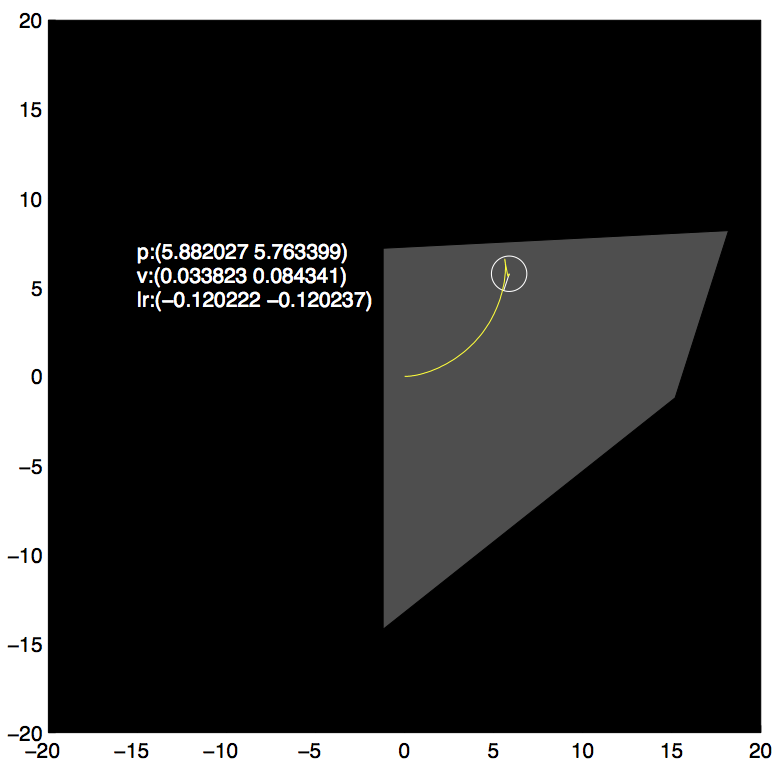
\includegraphics[width=\linewidth]{fig1.png}
    \captionsetup{singlelinecheck=off}
    \caption[.]{\label{fig:fig1}Simple trajectory \begin{align*}
    \omega_0 &= 0 \\
    \mathbf{v_0} &= (0, 0)\\
    \mathbf{d_0} &= (1, 0)
    \end{align*}
    }
\end{minipage}
\hfill
\begin{minipage}[t]{0.45\linewidth}
    \centering
    
    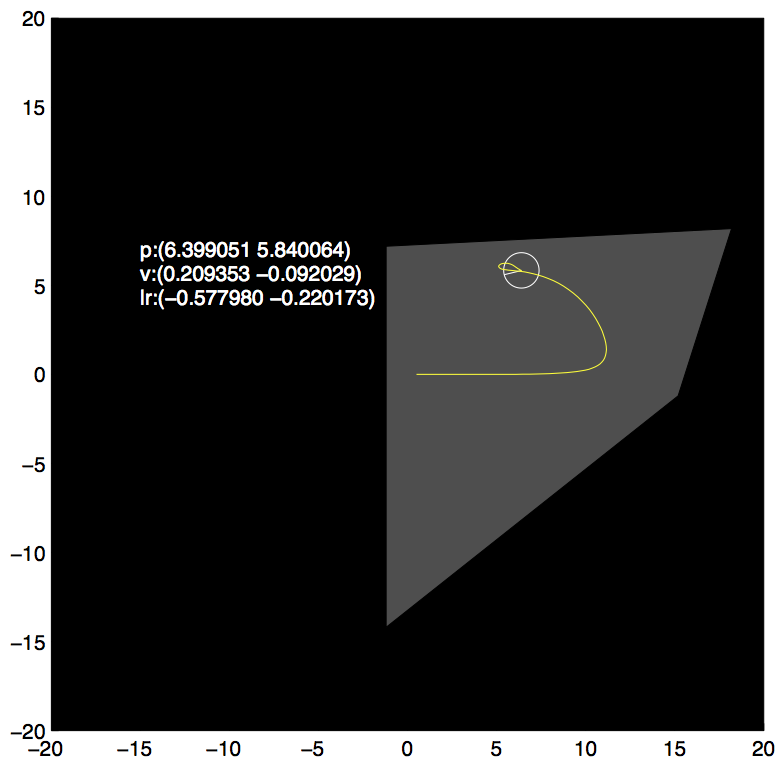
\includegraphics[width=\linewidth]{fig2.png}
    \captionsetup{singlelinecheck=off}
    \caption[.]{\label{fig:fig2}High initial velocity \begin{align*}
    \omega_0 &= 0 \\
    \mathbf{v_0} &= (3, 0)\\
    \mathbf{d_0} &= (1, 0)
    \end{align*}
    }\end{minipage}
\begin{minipage}[t]{0.45\linewidth}
    \centering
    
    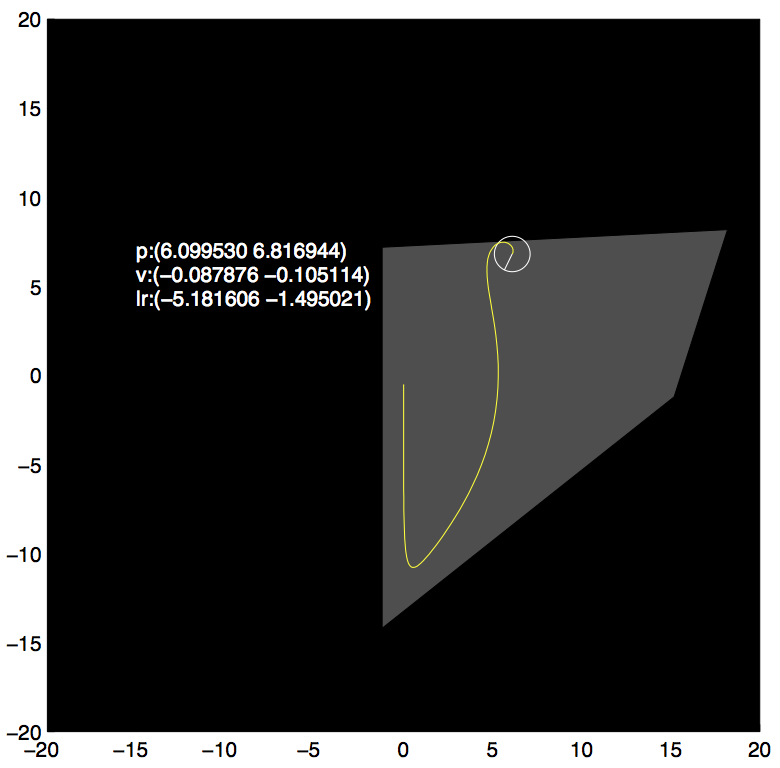
\includegraphics[width=\linewidth]{fig3.png}
    \captionsetup{singlelinecheck=off}
    \caption[.]{\label{fig:fig3}High initial velocity in the wrong direction\begin{align*}
    \omega_0 &= 0 \\
    \mathbf{v_0} &= (0, -2.5)\\
    \mathbf{d_0} &= (0, -1)
    \end{align*}
    }
\end{minipage}
\hfill
\begin{minipage}[t]{0.45\linewidth}
    \centering
    
    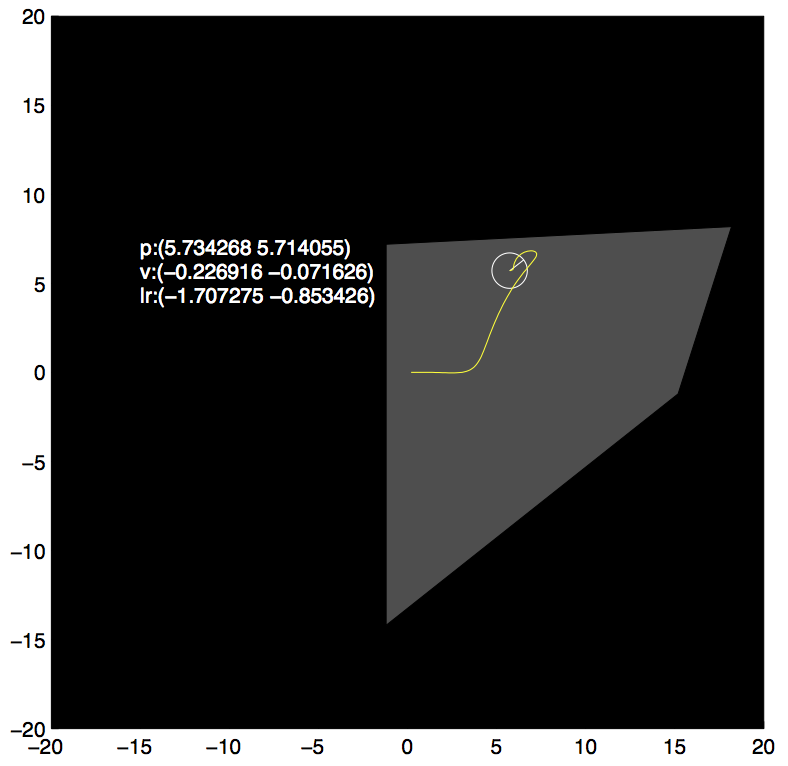
\includegraphics[width=\linewidth]{fig4.png}
    \captionsetup{singlelinecheck=off}
    \caption[.]{\label{fig:fig4}Initial rotation\begin{align*}
    \omega_0 &= 1 \\
    \mathbf{v_0} &= (0, 0)\\
    \mathbf{d_0} &= (1, 0)
    \end{align*}
    }
\end{minipage}
\end{minipage}
\end{figure}

\section{Other Implementations}
In the course of coming up with a solver for this problem, we tried other
types of algorithms that, for various reasons, failed to provide usable solutions.
\subsection{AMPL as a Solver}
Using a domain-specific tool like the AMPL programming language has benefits
when trying to solve non-linear constrained optimization problems because it
allows a much higher level description of the problem than a C solver, for instance.
Still, AMPL as a language is that it has a steep learning curve; AMPL (and the
resources available online) assumes that you are extremely comfortable with
formulating optimization
problems and even comfortable writing them in other languages. That being said
we did make some progress with specifying some optimization problems with it,
but the implementations are still lacking.

AMPL allowed us to make some leaps down the avenue of best-case optimization for
many sub-problems but was never completely integrated to provide a full problem
solution. However, since the main project itself was broken down into smaller
pieces, it seems appropriate that the level of AMPL code coincide with the
level of the project completeness. Therefore, the AMPL code was developed in
three distinct parts: simple movement in one direction with constrained velocity
and no acceleration; simple movement in one direction with constrained velocity
and acceleration with set time intervals; and simple rotation with constrained
velocity, acceleration, and moment of inertia. The three parts respectively optmized the
following variables: time, force input/output required, and energy.
Using these three development pathways we were able to solve some of the major
optimizing challenges, albeit separately.

The first pathway tries to examine how the tradeoff between time and energy
expenditure occurs while simply moving an object in a single direction. We set
the variables $N$ for discrete time intervals, time $t$, final position $\mathbf{x}_\text{final}$
and
scalar position coefficients $q$ and $r$. We then solve for the minimized force
tradeoff while moving the object, subject to the velocity and acceleration from
kinematic relationships. 

The second pathway allows for examining how an object needs to be constrained 
and tests minimizing time as opposed to energy expenditure (per movement). The
We set the parameters $\mathbf{x}_0$ and $\mathbf{x}_\text{final}$ for initial and
final position, $\mathbf{v}_0$ and $\mathbf{v}_\text{final}$ for
intial and final velocity and $\mathbf{x}_i$, $\mathbf{v}_i$, $\mathbf{a}_i$
for discretizations of position,
velocity, and acceleration respectively, for $1 \leq i \leq N$ where $N$
is the number of discrete
time intervals. We then subject those parameters to simple kinematics definitions
for velocity and acceleration and set the intial position and velocity vectors,
as well as intial conditions for number of steps, max speed, and max force.
Using these variables we solve, minimizing the total time $t$. 

The third pathway tries to solve the idea of trajectory setting with a radial
arm, since the project we are interested in solving uses a disc with a
paramaterized radius, the third pathway attempts to describe how to optimize
trajectory selection while optimizing least energy used, which is not the focus
of our problem, but provides at least some insite to how the problem can be 
tackled. It isn't a perfect model, and does not apply directly so there is no
need to go into more depth about it. However, it should be noted that this
experiment helped further understand how rotational kinematics can be optimized
in general.

\subsection{Symbolic Computation using Haskell}
Our initial attempt at computing the objective function and its gradient
involved attempting to find a closed-form symbolic expression that can be
rendered in C and evaluated relatively quickly. To this end, we made two attempts
at constructing a domain-specific language (DSL) embedded in the Haskell programming
language.

In the first attempt, we constructed a simple algebraic datatype for expressing
symbolic expressions containing variables. Optimization problems could be
expressed in a monadic context using quantifiers over arrays and recurrence
relations. Equality constraints are automatically eliminated via substitution,
and the calculation of the gradient is automatic. The resulting expressions can
be used to generate C or C++ code that detects common subexpressions, and
introduces sharing to make the computation as fast as possible. We tested this
on several test problems, such as computing a high-order best-fit polynomial,
minimizing a high-dimensional Rosenbrock function, and in each case were
pleased with the results. We used the same base L-BFGS solver code (using
\texttt{libLBFGS}) to optimize the generated objective function as the one we
ultimately used for the hand-coded objective function.

Although our toy functions worked very well in our tests, DSL proved no match
for the complexity of the trajectory objective function. The highly recursive
nature of the motion model means that to eliminate the equality constraints (i.e.,
the entire motion model), all references to position, velocity, and rotation
must be replaced by massive expressions dependent only on the $l_i$ and $r_i$
variables, and that is not even including any intermediate steps that we would
use to increase the accuracy of the differential equation solution (e.g., Runge-Kutta
or finite differences). Our DSL did in fact manage to compute the objective function
for this simplified case, although it failed to compute the gradient without
running out of memory.

Our second approach used a more clever model of storing expressions. Rather than
storing expressions in a tree and explicitly looking for common subexpressions
during code generation, we used the libraries \texttt{Data.Hashable} and \texttt{GHC.Generics}
to automatically generate hashes of expressions which are stored in an implicit
graph structure, so subexpression sharing is automatic. Using this method, our
objective function was able to be generated but the gradient was still too
large to be generated in a reasonable amount of time. In the interests of time,
we abandoned this approach in favour of the already-working hand-coded objective
function with numerical differentiation.

\chapter{Picking a Convex Subregion}
Now that we have a method for finding a trajectory within a convex subregion, we
need to find a way to integrate that into the larger problem.


\bibliographystyle{plain}
\bibliography{report}

\end{document}